%  CORONILLA
%  Texto y musica con acompa\~namiento by serachsam

% - Preambulo
\documentclass[12pt, letterpaper]{report}

%%% - Paquetes
\usepackage[spanish]{babel}
\usepackage[utf8]{inputenc}
\usepackage[T1]{fontenc}
\usepackage{xcolor}
\usepackage{pifont}
\usepackage{lettrine}
\usepackage{lmodern}
\usepackage{enumitem}
% Utilizamos el paquete para gestionar imagenes jpg
\usepackage{graphicx}
\graphicspath{ {images/} }
% hipervinculos
\usepackage{hyperref}

\oddsidemargin -1.0cm
\headsep -1.0cm
\textwidth=18.5cm
\textheight=23cm

\setlength{\parskip}{\baselineskip}

\setcounter{secnumdepth}{0}
\setcounter{tocdepth}{4}


%% Portada del Libro

%% Portada del Libro
\title{
  \textbf{ \Huge CORONILLA } \\
  \LARGE Rosario de la Virgen María \\
  \vspace{2em}
  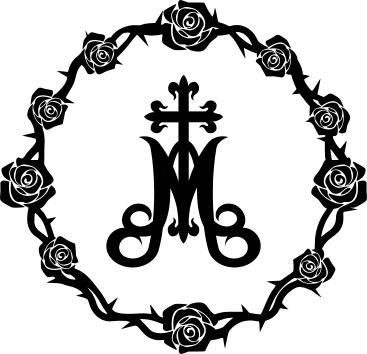
\includegraphics{rosa}
}

%\author{ \Large{ \textbf{Linda Isabel Mart\'inez Castro \\ Samuel Jos\'e Guti\'errez Avil\'es} } }

\author{ 
  \Large \textbf{Linda Isabel Mart\'inez Castro} \\ 
  \Large \textbf{Samuel Jos\'e Guti\'errez Avil\'es}
}

\date{ \LARGE \small \textit{2017 - 2019} }

\begin{document}
    %%\pagenumbering{gobble}
    %%\pagestyle{plain}

    %% - Portada
    \maketitle
    
    %% - Indice
    \LARGE ÍNDICE GENERAL

    \large \hfill{Página}\\
    \Large \textbf{Introducción \hfill{2}}\\
    .\hspace{1cm} \large Historia \dotfill 3\\
    .\hspace{1cm} \large Acerca del Rorasio y su Rezo \dotfill 3\\
    .\hspace{2cm} \large \textit{Historia del Rosario} \dotfill 3\\
    .\hspace{2cm} \large \textit{Indulgencias} \dotfill 6
    
    \noindent
    \Large \textbf{Rosario \hfill{8}}\\
    .\hspace{1cm} \large Ofrecimiento \dotfill 9\\
    .\hspace{1cm} \large Persignarse \dotfill 9\\
    .\hspace{1cm} \large Credo \dotfill 9\\
    .\hspace{1cm} \large Acto de Contrición \dotfill 9\\
    .\hspace{1cm} \large Anunciar el Misterio a Rezar \dotfill 10\\
    .\hspace{1cm} \large Padre Nuestro \dotfill 11\\
    .\hspace{1cm} \large Ave María \dotfill 12\\
    .\hspace{1cm} \large Gloria al Padre \dotfill 12\\
    .\hspace{1cm} \large Letanías de la Virgen María \dotfill 12\\
    .\hspace{1cm} \large La Salve \dotfill 12\\
    .\hspace{1cm} \large Oración al Final \dotfill 12
    \clearpage

    %% - Introduccion
    \begin{center}
        \vspace*{9cm}
        \textbf{\Huge Introducci\'on}
    \end{center}
    \clearpage
    
    \LARGE HISTORIA
    
    \Large Esta música nació de las ganas no caer en la monotonía al rezar el Rosario. Un d\'ia simplemente pensamos: <<?`Porque no lo hacemos cantado?>> Recordamos diferente tonos que habíamos escuchado que se cantaban las diferentes partes, pero no había una melodía o tono coherente en todo el recorrido del rezo. Sin más nos decidimos de hacer una melodía completa.
    
    Junto con escuchar las diferentes versiones gregorianas e investigar que textos se musicalizarian nos decidimos por hacer un sola melodía homogenia para todo el <<Rosario>>, que fuera fácil de interpretar y de recordar.
    
    \LARGE ACERCA DEL ROSARIO Y SU REZO
    
    \LARGE \textit{Historia del Rosario}
    
    \Large Existen diversas explicaciones sobre como surgió el rezo de <<El Rosario>>, todas validas y loables, como esta:
    
    \Large \textit{<<En la antigüedad, los romanos y los griegos solían coronar con rosas a las estatuas que representaban a sus dioses como símbolo del sufrimiento de sus corazones. Siguiendo esta tradición, las mujeres cristianas que eran llevadas al martirio por los romanos, marchaban por el coliseo vestidas con sus ropas más vistosas y con sus cabezas adornadas con coronas de rosas, como símbolo de alegría y de la entrega de sus corazones al ir al encuentro de Dios. Por la noche, los cristianos recogían sus coronas y por cada rosa, recitaban una oración o un salmo por el eterno descanso del alma de las mártires por eso se llama Rosario. La palabra ``Rosario'' significa ``Corona de Rosas''. La Iglesia recomendó rezar el ``Rosario'', el cual consistía en recitar los 150 salmos de David, pues era considerada una oración sumamente agradable a Dios y fuente de innumerables gracias para aquellos que la rezaran. Sin embargo, esta recomendación sólo la seguían las personas cultas y letradas, pero no la mayoría de los cristianos. Por esto, la Iglesia sugirió que aquellos que no supieran leer, suplantaran los 150 salmos por 150 Avemarías, divididas en quince decenas. A este ``Rosario corto'' se le llamó ``El salterio de la Virgen''.>>} \cite{RorasioCatholicNet}
    
    \Large O esta otra:
    
    \Large \textit{<<El rezo del ``Santo Rosario'' surge aproximadamente en el año 800 a la sombra de los monasterios, como ``Salterio de los laicos''. Dado que los monjes rezaban los 150 salmos de David, a los laicos, los cuales en su mayoría no sabían leer, se les enseñó a rezar 150 Padres Nuestros. Al pasar el tiempo, se formaron otros tres salterios con 150 Aves Marías, 150 alabanzas en honor de Jesús y 150 alabanzas en honor de María. En el año 1365 se hizo una combinación de los cuatro salterios, dividiendo las 150 Aves Marías en 15 decenas y poniendo un Padre nuestro al inicio de cada una de ellas. En 1500 se estableció, para cada decena, la meditación de un hecho de la vida de Jesús o María, y así surgió el actual Rosario de quince misterios. La palabra Rosario significa ``Corona de Rosas''. La Virgen María ha revelado a muchas personas que cada vez que rezan un Ave María le entregan una rosa y por cada Rosario completo le entregan una corona de rosas. La rosa es la reina de las flores, así que el Rosario es la rosa de todas las devociones y por lo tanto es la más importante.>>}\cite{AciPrensaRosario}
    
    \Large Dependiendo de la fuente que se consulte, pero es cierto que su devoción empezó así:
    
    \Large \textit{<<A finales del siglo XII, se le apareció la Virgen a Santo Domingo de Guzmán y le dijo que la mejor arma para convertir a las almas duras no era con el rezo de su salterio. Santo Domingo realizo varios milagros Toulouse mientras rezar el salterio de la Virgen convirtiendo muchas personas. Santo Domingo murió en 1221, después de una vida en la que se dedicó a predicar y hacer popular la devoción del <<Rosario>> entre las gentes de todas las clases sociales para el sufragio de las almas del Purgatorio, para el triunfo sobre el mal y prosperidad de la Santa Madre de la Iglesia. El rezo del Rosario mantuvo su fervor por cien años después de la muerte de Santo Domingo y empezó a ser olvidado. En 1349, hubo en Europa una terrible epidemia de peste a la que se le llamó ``La muerte negra'' en la que murieron muchísimas personas. Fue entonces cuando el fraile Alan de la Roche, superior de los dominicos en la misma provincia de Francia donde había comenzado la devoción al Rosario, tuvo una aparición, en la cual Jesús, la Virgen y Santo Domingo le pidieron que reviviera la antigua costumbre del rezo del Santo Rosario. El Padre Alan comenzó esta labor de propagación junto con todos los frailes dominicos en 1460. Ellos le dieron la forma que tiene actualmente, con la aprobación eclesiástica. A partir de entonces, esta devoción se extendió en toda la Iglesia.>>}\cite{RorasioCatholicNet}
    
    \Large Y que en la actualidad la iglesia ve <<El Rosario>> de esta manera:
    
    \Large ``El Rosario de la Virgen María, difundido gradualmente en el segundo Milenio bajo el soplo del Espíritu de Dios, es una oración apreciada por numerosos Santos y fomentada por el Magisterio. En su sencillez y profundidad, sigue siendo también en este tercer Milenio apenas iniciado una oración de gran significado, destinada a producir frutos de santidad. Se encuadra bien en el camino espiritual de un cristianismo que, después de dos mil años, no ha perdido nada de la novedad de los orígenes, y se siente empujado por el Espíritu de Dios a «remar mar adentro» (duc in altum!), para anunciar, más aún, 'proclamar' a Cristo al mundo como Señor y Salvador, «el Camino, la Verdad y la Vida» (Jn14, 6), el «fin de la historia humana, el punto en el que convergen los deseos de la historia y de la civilización». El Rosario, en efecto, aunque se distingue por su carácter mariano, es una oración centrada en la cristología. En la sobriedad de sus partes, concentra en sí la profundidad de todo el mensaje evangélico, del cual es como un compendio. En él resuena la oración de María, su perenne Magnificat por la obra de la Encarnación redentora en su seno virginal. Con él, el pueblo cristiano aprende de María a contemplar la belleza del rostro de Cristo y a experimentar la profundidad de su amor. Mediante el Rosario, el creyente obtiene abundantes gracias, como recibiéndolas de las mismas manos de la Madre del Redentor.''\cite{Enciclica}
    
    \LARGE \textit{Indulgencias}
    
    \Large ``Para fomentar esta proyección eclesial del Rosario, la Iglesia ha querido enriquecerlo con santas indulgencias para quien lo recita con las debidas disposiciones.''\cite{Enciclica}
    
    Es tan grande el aprecio que la Iglesia ha tenido por el Rezo del Rosario que los Papas han concedido muchas indulgencias a lo largo de la historia. A continuación Detallaremos algunas:

    \begin{enumerate}
      \item Se concede indulgencia plenaria al fiel cristiano que:
      \begin{itemize}
        \item Rece devotamente el Rosario mariano en una iglesia u oratorio, o en familia, en una comunidad religiosa, en una asociación piadosa y, en general, en cualquier reunión de fieles.\cite{Indulgencias}
        \item Se una devotamente al rezo de esta plegaria llevado a cabo por el Sumo Pontífice y retransmitida por radio o por televisión.\cite{Indulgencias}
      \end{itemize}
      \item El fiel cristiano puede ganar una indulgencia si usa con devoción algún objeto de piedad (crucifijo o cruz, rosario, escapulario, medalla) debidamente bendecido.
      \item Son dignas de especial mención las concesiones que se refieren a algunas obras, enriquecidas con indulgencia plenaria, con las cuales el fiel cristiano puede ganarla todos los días del año:
      \begin{itemize}
        \item La adoración del Santísimo Sacramento durante al menos media hora.\cite{Indulgencias}
        \item El piadoso ejercicio del Via Crucis.\cite{Indulgencias}
        \item El rezo del Rosario mariano o del himno Akhátistos en una iglesia o un oratorio, o en familia, en una comunidad religiosa, en una asociación piadosa y, en general, siempre que varios fieles se reúnan para un buen fin.\cite{Indulgencias}
        \item La lectura piadosa de la Sagrada Escritura durante al menos media hora.\cite{Indulgencias}
      \end{itemize}
    \end{enumerate}
    \clearpage
    
    %% - Rosario
    \begin{center}
        \vspace*{8cm}
        \textbf{\Huge Santo Rosario}\\
        \vspace*{1cm}
        \Large Rezar el Rosario de la Virgen María\cite{VaticanRosary}
    \end{center}
    \clearpage
    
    \LARGE 1. Ofrecimiento
    
    \Large Intención por la cual se reza el rosario, puede ser por un difunto, las animas del Purgatorio o una situación en particular; para pedir una gracia, una virtud a imitar o un pecado a evitar. Puede hacerse en silencio si se reza solo.
    
    \textit{<<Ofrezco(Ofrecemos) el rezo de este rosario por: ...>>}
    
    \LARGE 2. Persignarse
    
    \Large Hacer la señal de la cruz sobre la frente, la cara y el pecho. 
    
    \textit{<<Por la señal de la Santa Cruz, de nuestros enemigos líbranos Señor, Dios nuestro. En el nombre del Padre, y del Hijo y del Espíritu Santo. Amén.>>}
    
    %\begin{lilypond}%[staffsize=20]
    %  \include "../write/persignarse/persignarse.ly"
    %\end{lilypond}
    %\clearpage
    
    \LARGE 3. Credo
    
    \Large Sujetando el <<Rosario>> por el crucifijo se reza el Credo Apostólico.
    
    \textit{<<Creo en Dios, Padre todopoderoso, Creador del cielo y de la tierra.\\
    Creo en Jesucristo, su único Hijo, nuestro Señor, que fue concebido por obra y gracia del Espíritu Santo, nació de Santa María Virgen, padeció en tiempos de Poncio Pilato, fue crucificado, muerto y sepultado, descendió a los infiernos, al tercer día resucitó de entre los muertos, subió a los cielos y está sentado a la derecha de Dios, Padre todopoderoso. Desde allí ha de venir a juzgar a vivos y muertos.\\
    Creo en el Espíritu Santo, la santa Iglesia Católica, la comunión de los santos, el perdón de los pecados, la resurrección de la carne y la vida eterna. Amén.>>}
    
    %\begin{lilypond}%[staffsize=20]
    %    \include "../write/credo/credo.ly"
    %\end{lilypond}
    %\clearpage
    
    \LARGE 3. Acto de contrición
    
    \Large Apoyamos la costumbre de agregar el rezo del acto de contrición al Rosario. Existen diversas oraciones del penitente, las más común el <<Yo Confieso>>, cualquiera es valida, pero usaremos la siguiente:
    
    \textit{<<¡Señor mío, Jesucristo! Dios y Hombre verdadero, Creador, Padre y Redentor mío; por ser Vos quien sois, Bondad infinita, y porque os amo sobre todas las cosas, me pesa de todo corazón haberos ofendido; también me pesa porque podéis castigarme con las penas del infierno. Ayudado de vuestra divina gracia propongo firmemente nunca más pecar, confesarme y cumplir la penitencia que me fuere impuesta. Amén.>>}
    
    %\begin{lilypond}%[staffsize=20]
    % \include "../write/acto_contriccion/acto_contriccion.ly"
    %\end{lilypond}
    %\clearpage
    
    \LARGE 4. Anunciar el Misterio a Rezar
    
    \Large El rosario consta de de veinte Misterios y están ordenados en cuatro grupos. A cada grupo le corresponde un día de la semana (Igualmente se puede rezar todos lo misterios en un solo día).
    
    \begin{enumerate}
        \item \textsc{Misterios de Gozo}: \textit{Lunes y Sábado}
        \begin{itemize}
         \item La encarnación del Hijo de Dios: \textit{Lucas 1, 26-38}
         \item La visita de la Virgen María a su prima Isabel: \textit{Lucas 1, 39-43}
         \item El nacimiento del Hijo de Dios en Belén: \textit{Lucas 2, 1-7}
         \item La presentación de Jesús en el templo: \textit{Lucas 2, 21-25}
         \item El niño Jesús perdido y hallado en el templo: \textit{Lucas 2, 41-47}
        \end{itemize}
        \item \textsc{Misterios de Luz}: \textit{Jueves}
        \begin{itemize}
         \item El bautismo del Señor en el Jordán: \textit{Mateo 3, 16-17}
         \item Las bodas de Caná: \textit{Juan 2, 1-5}
         \item El anuncio del Reino de Dios: \textit{Marcos 1, 15}
         \item La Transfiguración: \textit{Mateo 17, 1-5}
         \item La institución de la Eucaristía: \textit{Mateo 26, 26-29}
        \end{itemize}
        \item \textsc{Misterios de Dolor}: \textit{Martes y Viernes}
        \begin{itemize}
         \item La oración de Jesús en el Huerto: \textit{Mateo 26, 36-39}
         \item La flagelación de Jesús atado a la columna: \textit{Juan 19, 1-3}
         \item La coronación de espinas: \textit{Mateo 27, 27-29}
         \item Jesús con la cruz a cuestas camino del Calvario: \textit{Marcos 15, 21-22}
         \item La crucifixión y muerte de Jesús: \textit{Lucas 23, 33-46}
        \end{itemize}
        \item \textsc{Misterios de Gloria}: \textit{Miércoles y Domingo}
        \begin{itemize}
         \item La Resurrección del Hijo de Dios: \textit{Lucas 24, 1-6}
         \item La Ascensión del Señor al cielo: \textit{Marcos 16, 19-20}
         \item La venida del Espíritu Santo: \textit{Hechos de los Apostóles 2, 1-4}
         \item La Asunción de María al cielo: \textit{Lucas 1, 48-49}
         \item La Coronación de María como Reina: \textit{Apocalipsis 12, 1}
        \end{itemize}
    \end{enumerate}
        
    \textit{<<Hoy rezaremos los misterios de ...>>}
    
    Y según el día se anuncia uno a uno los misterios del día.

    \textit{<<El Primer/Segundo/Tercer/Cuarto/Quinto misterio\\ de Gozo/Luz/Dolor/Gloria es ...>>}
    
    Cada misterios se consta de un Padre Nuestro y diez Ave Marías. Es recomendable leer la cita bíblica y luego meditar la palabra.

    \LARGE 5. Padre Nuestro
    
    \Large Al inicio de casa misterio se reza un Padre Nuestro.
    
    \textit{<<Padre nuestro, que estás en el cielo, santificado sea tu nombre; venga a nosotros tu reino; hágase tu voluntad, en la tierra como en el cielo. Danos hoy nuestro pan de cada día; perdona nuestras ofensas, como también nosotros perdonamos a los que nos ofenden; no nos dejes caer en la tentación, y líbranos del mal. Amén.>>}
    
    %\begin{lilypond}%[staffsize=20]
    %    \include "../write/padre_nuestro/padre_nuestro.ly"
    %\end{lilypond}
    %\clearpage
    
    \LARGE 6. Ave María
    
    \Large En cada misterio se rezan diez Ave María.
    
    \textit{<<Dios te Salve, María, llena eres de gracia; el Señor es contigo. Bendita tú eres entre todas las mujeres, y bendito es el fruto de tu vientre, Jesús. Santa María, Madre de Dios, ruega por nosotros, pecadores, ahora y en la hora de nuestra muerte. Amén.>>}
    
    %\begin{lilypond}%[staffsize=20]
    %    \include "../write/ave_maria/ave_maria.ly"
    %\end{lilypond}
    %\clearpage
    
    \LARGE 7. Gloria al Padre
    
    \Large Luedo de las diez Ave María se reza un Gloria al Padre.
    
    \textit{<<Gloria al Padre y al Hijo y al Espíritu Santo. Como era en el principio, ahora y siempre, por los siglos de los siglos. Amén.>>}
    
    \LARGE 8. Jaculatoria
    
    \Large La Jaculatoria final varía según las costumbres del lugar, nosotros recomendaremos las siguientes:
    
    \textsc{Oración de Fátima}\\
    \textit{<<Oh Jesús mío, perdona nuestros pecados, líbranos del fuego del infierno, lleva al cielo a todas las almas, especialmente a las más necesitadas de tu misericordia.>>}
    
    \textsc{Madre de Gracia}\\
    V/. \textit{<<María, Madre de Gracia, Madre de Misericordia.>>}\\R/. \textit{<<En la vida y en la muerte ampáranos Gran Señora.>>}
    
    \textsc{Oración de Cuapa}\\
    \textit{<<Santísima Virgen María, tú eres mi madre la madre de todos nosotros los pecadores.>>}
    
    \Large Los puntos del 4. al 8. se repetirán hasta completar los misterios, ya sean los del día o los elegidos a rezar.
    
    \LARGE 8. Rezar por la intenciones del Papa
    
    \Large Se reza un Padre Nuestro, tres Ave María y un Gloria al Padre por las intenciones del Papa.
    
    \textit{<<Ahora rezamos por as intenciones del Santo Padre: ...>>}
    
    \textit{<<Padre nuestro...>>}

    Las Ave María se cambian un poco para realzar los dogma de María.
    
    \textbf{1.} \textit{<<Dios te Salve, María, virgen antes del parto, alcánzanos la virtud de la Fe, llena eres de gracia...>>}
    
    \textbf{2.} \textit{<<Dios te Salve, María, virgen durante del parto, alcánzanos la virtud de la Esperanza, llena eres de gracia...>>}
    
    \textbf{3.} \textit{<<Dios te Salve, María, virgen después del parto, alcánzanos la virtud de la Caridad, llena eres de gracia...>>}
    
    \textit{<<Gloria al Padre...>>}
        
    \LARGE 9. Letanías de la Virgen María
    
    \Large \hfill{Respuesta}\\
    \Large V/. \textit{<<Señor, ten piedad.>>} \hfill{R/. \textit{<<Señor, ten piedad.>>}}\\
    \Large V/. \textit{<<Cristo, ten piedad.>>} \hfill{R/. \textit{<<Cristo, ten piedad.>>}}\\
    \Large V/. \textit{<<Señor, ten piedad.>>} \hfill{R/. \textit{<<Señor, ten piedad.>>}}\\
    \Large V/. \textit{<<Cristo, escúchanos.>>} \hfill{R/. \textit{<<Cristo, escúchanos.>>}}
    
    \noindent
    \Large V/. \textit{<<Dios, Padre celestial.>>} \hfill{R/. \textit{<<Ten piedad de nosotros.>>}}\\
    \Large V/. \textit{<<Dios, Hijo, Redentor del mundo.>>} \hfill{R/. \textit{<<Ten piedad de nosotros.>>}}\\
    \Large V/. \textit{<<Dios, Espíritu Santo.>>} \hfill{R/. \textit{<<Ten piedad de nosotros.>>}}\\
    \Large V/. \textit{<<Santísima Trinidad, un solo Dios.>>} \hfill{R/. \textit{<<Ten piedad de nosotros.>>}}
    
    \noindent
    \Large V/. \textit{<<Santa María.>>} \hfill{R/. \textit{<<Ruega por nosotros.>>}}\\
    \Large V/. \textit{<<Santa Madre de Dios.>>} \hfill{R/. \textit{<<Ruega por nosotros.>>}}\\
    \Large V/. \textit{<<Santa Virgen de las Vírgenes.>>} \hfill{R/. \textit{<<Ruega por nosotros.>>}}\\
    \Large V/. \textit{<<Madre de Cristo.>>} \hfill{R/. \textit{<<Ruega por nosotros.>>}}\\
    \Large V/. \textit{<<Madre de la Iglesia.>>} \hfill{R/. \textit{<<Ruega por nosotros.>>}}\\
    \Large V/. \textit{<<Madre de la misericordia.>>} \hfill{R/. \textit{<<Ruega por nosotros.>>}}\\
    \Large V/. \textit{<<Madre de la divina gracia.>>} \hfill{R/. \textit{<<Ruega por nosotros.>>}}\\
    \Large V/. \textit{<<Madre de la esperanza.>>} \hfill{R/. \textit{<<Ruega por nosotros.>>}}\\
    \Large V/. \textit{<<Madre purísima.>>} \hfill{R/. \textit{<<Ruega por nosotros.>>}}\\
    \Large V/. \textit{<<Madre castísima.>>} \hfill{R/. \textit{<<Ruega por nosotros.>>}}\\
    \Large V/. \textit{<<Madre siempre virgen.>>} \hfill{R/. \textit{<<Ruega por nosotros.>>}}\\
    \Large V/. \textit{<<Madre inmaculada.>>} \hfill{R/. \textit{<<Ruega por nosotros.>>}}\\
    \Large V/. \textit{<<Madre amable.>>} \hfill{R/. \textit{<<Ruega por nosotros.>>}}\\
    \Large V/. \textit{<<Madre admirable.>>} \hfill{R/. \textit{<<Ruega por nosotros.>>}}\\
    \Large V/. \textit{<<Madre del buen consejo.>>} \hfill{R/. \textit{<<Ruega por nosotros.>>}}\\
    \Large V/. \textit{<<Madre del Creador.>>} \hfill{R/. \textit{<<Ruega por nosotros.>>}}\\
    \Large V/. \textit{<<Madre del Salvador.>>} \hfill{R/. \textit{<<Ruega por nosotros.>>}}\\
    \Large V/. \textit{<<Virgen prudentísima.>>} \hfill{R/. \textit{<<Ruega por nosotros.>>}}\\
    \Large V/. \textit{<<Virgen digna de veneración.>>} \hfill{R/. \textit{<<Ruega por nosotros.>>}}\\
    \Large V/. \textit{<<Virgen digna de alabanza.>>} \hfill{R/. \textit{<<Ruega por nosotros.>>}}\\
    \Large V/. \textit{<<Virgen poderosa.>>} \hfill{R/. \textit{<<Ruega por nosotros.>>}}\\
    \Large V/. \textit{<<Virgen clemente.>>} \hfill{R/. \textit{<<Ruega por nosotros.>>}}\\
    \Large V/. \textit{<<Virgen fiel.>>} \hfill{R/. \textit{<<Ruega por nosotros.>>}}\\
    \Large V/. \textit{<<Espejo de justicia.>>} \hfill{R/. \textit{<<Ruega por nosotros.>>}}\\
    \Large V/. \textit{<<Trono de la sabiduría.>>} \hfill{R/. \textit{<<Ruega por nosotros.>>}}\\
    \Large V/. \textit{<<Causa de nuestra alegría.>>} \hfill{R/. \textit{<<Ruega por nosotros.>>}}\\
    \Large V/. \textit{<<Vaso espiritual.>>} \hfill{R/. \textit{<<Ruega por nosotros.>>}}\\
    \Large V/. \textit{<<Vaso digno de honor.>>} \hfill{R/. \textit{<<Ruega por nosotros.>>}}\\
    \Large V/. \textit{<<Vaso de insigne devoción.>>} \hfill{R/. \textit{<<Ruega por nosotros.>>}}\\
    \Large V/. \textit{<<Rosa mística.>>} \hfill{R/. \textit{<<Ruega por nosotros.>>}}\\
    \Large V/. \textit{<<Torre de David.>>} \hfill{R/. \textit{<<Ruega por nosotros.>>}}\\
    \Large V/. \textit{<<Torre de marfil.>>} \hfill{R/. \textit{<<Ruega por nosotros.>>}}\\
    \Large V/. \textit{<<Casa de oro.>>} \hfill{R/. \textit{<<Ruega por nosotros.>>}}\\
    \Large V/. \textit{<<Arca de la Alianza.>>} \hfill{R/. \textit{<<Ruega por nosotros.>>}}\\
    \Large V/. \textit{<<Puerta del cielo.>>} \hfill{R/. \textit{<<Ruega por nosotros.>>}}\\
    \Large V/. \textit{<<Estrella de la mañana.>>} \hfill{R/. \textit{<<Ruega por nosotros.>>}}\\
    \Large V/. \textit{<<Salud de los enfermos.>>} \hfill{R/. \textit{<<Ruega por nosotros.>>}}\\
    \Large V/. \textit{<<Refugio de los pecadores.>>} \hfill{R/. \textit{<<Ruega por nosotros.>>}}\\
    \Large V/. \textit{<<Consuelo de los migrantes.>>} \hfill{R/. \textit{<<Ruega por nosotros.>>}}\\
    \Large V/. \textit{<<Consoladora de los afligidos.>>} \hfill{R/. \textit{<<Ruega por nosotros.>>}}\\
    \Large V/. \textit{<<Auxilio de los cristianos.>>} \hfill{R/. \textit{<<Ruega por nosotros.>>}}\\
    \Large V/. \textit{<<Reina de los Ángeles.>>} \hfill{R/. \textit{<<Ruega por nosotros.>>}}\\
    \Large V/. \textit{<<Reina de los Patriarcas.>>} \hfill{R/. \textit{<<Ruega por nosotros.>>}}\\
    \Large V/. \textit{<<Reina de los Profetas.>>} \hfill{R/. \textit{<<Ruega por nosotros.>>}}\\
    \Large V/. \textit{<<Reina de los Apóstoles.>>} \hfill{R/. \textit{<<Ruega por nosotros.>>}}\\
    \Large V/. \textit{<<Reina de los Mártires.>>} \hfill{R/. \textit{<<Ruega por nosotros.>>}}\\
    \Large V/. \textit{<<Reina de los Confesores.>>} \hfill{R/. \textit{<<Ruega por nosotros.>>}}\\
    \Large V/. \textit{<<Reina de las Vírgenes.>>} \hfill{R/. \textit{<<Ruega por nosotros.>>}}\\
    \Large V/. \textit{<<Reina de todos los Santos.>>} \hfill{R/. \textit{<<Ruega por nosotros.>>}}\\
    \Large V/. \textit{<<Reina concebida sin pecado original.>>} \hfill{R/. \textit{<<Ruega por nosotros.>>}}\\
    \Large V/. \textit{<<Reina asunta a los Cielos.>>} \hfill{R/. \textit{<<Ruega por nosotros.>>}}\\
    \Large V/. \textit{<<Reina del Santísimo Rosario.>>} \hfill{R/. \textit{<<Ruega por nosotros.>>}}\\
    \Large V/. \textit{<<Reina de la familia.>>} \hfill{R/. \textit{<<Ruega por nosotros.>>}}\\
    \Large V/. \textit{<<Reina de la paz.>>} \hfill{R/. \textit{<<Ruega por nosotros.>>}}
    
    \noindent
    \Large V/. \textit{<<Cordero de Dios, que quitas el pecado del mundo.>>}\\ R/. \textit{<<Perdónanos, Señor.>>}\\
    \Large V/. \textit{<<Cordero de Dios, que quitas el pecado del mundo.>>}\\
    R/. \textit{<<Escúchanos, Señor.>>}\\
    \Large V/. \textit{<<Cordero de Dios, que quitas el pecado del mundo.>>}\\
    R/. \textit{<<Ten misericordia de nosotros.>>}
    
    \noindent
    \Large V/. \textit{<<Ruega por nosotros, Santa Madre de Dios.>>}\\
    R/. \textit{<<Para que seamos dignos de las promesas de Cristo.>>}
    
    
    %\begin{lilypond}%[staffsize=20]
    %  \include "../write/letanias/letanias.ly"
    %\end{lilypond}
    %\clearpage
    
    \LARGE 10. La Salve
    
    \Large \textsc{Salve Regina}\\
    \textit{<<Dios te salve, Reina y Madre de misericordia, vida, dulzura y esperanza nuestra; Dios te salve. A Ti llamamos los desterrados hijos de Eva; a Ti suspiramos gimiendo y llorando, en este valle de lágrimas. Ea, pues, Señora abogada nuestra, vuelve a nosotros esos tus ojos misericordiosos; y después de este destierro muéstranos a Jesús, fruto bendito de tu vientre. ¡Oh clemente, oh piadosa, oh dulce siempre Virgen María!>>}

    \Large \textsc{Oración Final}\\
    V/. \textit{<<Ruega por nosotros, Santa Madre de Dios>>}\\
    R/. \textit{<<Para que seamos dignos de alcanzar las promesas de Nuestro Señor Jesucristo. Amén.>>}
    
    %\begin{lilypond}%[staffsize=20]
    %    \include "../write/salve/salve.ly"
    %\end{lilypond}
    %\clearpage
    
    \LARGE 10. Oración al final
    
    \Large Puede añadir una o más oraciones al final. Nosotro usaremos:
    
    \textit{<<Te rogamos nos concedas, Señor Dios nuestro, gozar de continua salud de alma y cuerpo, y por la gloriosa intercesión de la bienaventurada siempre Virgen María, vernos libres de las tristezas de la vida presente y disfrutar de las alegrías eternas. Por Cristo nuestro Señor. Amén.>>}
    
    %\begin{lilypond}%[staffsize=20]
    %    \include "../write/oracion_final/oracion_final.ly"
    %\end{lilypond}
    %\clearpage
    
    \begin{thebibliography}{0}
      \bibitem{RorasioCatholicNet} \href{http://www.rosario.catholic.net/index.php}{\textsc{Catholic.net}: ¿Qué es el Santo Rosario?}
      
      \bibitem{AciPrensaRosario} \href{https://www.aciprensa.com/Rosario/surgio.htm}{\textsc{AciPrensa.com}: Como surgió el rezo del Santo Rosario}

      \bibitem{Enciclica} \href{https://www.vatican.va/content/john-paul-ii/es/apost_letters/2002/documents/hf_jp-ii_apl_20021016_rosarium-virginis-mariae.html}{\textsc{Vatican.va}: Carta Apostólica Rosarium Virginis Mariae}

      \bibitem{Indulgencias} \href{https://liturgiapapal.org/attachments/article/1076/Indulgencias.pdf}{\textsc{LiturgiaPapal.org}: Manual de Indulgencias}
 
      \bibitem{VaticanRosary} \href{https://www.vatican.va/special/rosary/index_rosary_sp.htm}{\textsc{Vatican.va}: El Santo Rosario}

    \end{thebibliography}
\end{document}
 
